\begin{figure}[H]
    \centering
    \definecolor{deformblue}{RGB}{40,115,185}
    \definecolor{initialgray}{RGB}{115,120,125}
    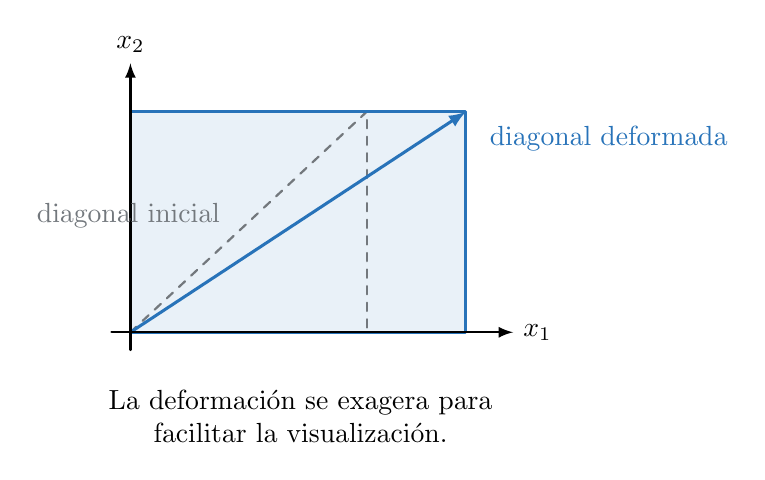
\begin{tikzpicture}[x=3.0cm,y=2.8cm,line cap=round,line join=round]
        \fill[deformblue!10] (0,0) -- (1.42,0) -- (1.42,1) -- (0,1) -- cycle;
        \draw[initialgray,dashed,line width=0.8pt] (0,0) rectangle (1,1);
        \draw[initialgray,dashed,line width=0.8pt] (0,0) -- (1,1);
        \draw[deformblue,line width=1pt] (0,0) rectangle (1.42,1);
        \draw[deformblue,-latex,line width=1.1pt] (0,0) -- (1.42,1);
        \draw[-latex,line width=0.8pt] (-0.08,0) -- (1.62,0) node[right] {$x_1$};
        \draw[-latex,line width=0.8pt] (0,-0.08) -- (0,1.22) node[above] {$x_2$};
        \node[initialgray,above left] at (0.42,0.43) {diagonal inicial};
        \node[deformblue,anchor=west] at (1.48,0.88) {diagonal deformada};
        \node[align=center] at (0.72,-0.38) {La deformación se exagera para\\facilitar la visualización.};
    \end{tikzpicture}
    \caption{La cara $x_1x_2$ se alarga en la dirección $x_1$, aumentando su diagonal.}
\end{figure}